\documentclass{article}

% Eshtetic packages -----------------------
\usepackage{geometry}
 \geometry{
 a4paper,
 total={170mm,257mm},
 left=25mm,
 right=25mm,
 top=25mm,
 bottom=25mm,
 }

 % A little black magic
\usepackage{microtype}

% Other Packages --------------------------

\usepackage{stmaryrd}
\usepackage{biblatex}
\usepackage[T1]{fontenc}
\usepackage{enumitem}

\usepackage{graphicx}
\graphicspath{ {../images/} }


\usepackage{caption}
\usepackage{subcaption}
\usepackage{amsthm}
\usepackage{amsmath}
\usepackage{amssymb}
\usepackage[french]{babel}
% \usepackage[autolanguage]{numprint} % for the \nombre command
\usepackage{hyphenat}
% \usepackage{minted}
% \setminted[ocaml]{style=vs}

\usepackage{tikz}
\usetikzlibrary[cd]

% Operators -------------------------------

\let\loop\relax
\DeclareMathOperator{\loop}{loop}
\DeclareMathOperator{\inv}{inv}
\DeclareMathOperator{\isconnected}{is-connected}
\DeclareMathOperator{\isgroupoid}{is-groupoid}
\let\Pr\relax
\DeclareMathOperator{\Pr}{Pr}
\DeclareMathOperator{\shape}{shape}
\DeclareMathOperator{\gset}{G-Set}
\DeclareMathOperator{\torsor}{Torsor}
\DeclareMathOperator{\aut}{Aut}
\DeclareMathOperator{\code}{code}
\DeclareMathOperator{\decode}{decode}
\DeclareMathOperator{\transport}{transport}
\DeclareMathOperator{\refl}{refl}
\DeclareMathOperator{\baut}{BAut}
\DeclareMathOperator{\set}{Set}
\DeclareMathOperator{\prop}{Prop}
\DeclareMathOperator{\groupa}{Group}
\let\hom\relax
\DeclareMathOperator{\hom}{Hom}

% \addbibresource{bibliographie.bib}

% \captionsetup{labelformat=empty}

%\renewcommand{\labelitemi}{$\bullet$}

\newtheorem{definition}{Définition}[section]
\newtheorem{theorem}{Théorème}[section]
\newtheorem{proposition}[definition]{Proposition}
\newtheorem{lemme}[definition]{Lemme}
% \newtheorem{conjecture}[definition]{Conjecture}
% \newtheorem{exemple}[definition]{Exemple}


\title{Construction des espaces de Eilenberg-MacLane en HoTT}

\author{Stage L3 de Camil Champin}
\author{Camil Champin\\[1ex]
\small Encadré par Emile Oleon et Samuel Mimram}  % use a smaller font size
\date{Juin-Juillet 2023}

\begin{document}

\maketitle

\section{Introduction du problème}

\subsection{Espaces d'Eilenberg-MacLane}

% Ceci devrait s'écrire tout seul
%

On dispose d'un groupe $G$ et on cherche à construire un espace, dit de \emph{Eilenberg-Maclane}, dont le groupe fondamental sera $G$, et dont tout les autres groupes d'homotopie seront triviaux. On dis qu'un tel espace est un $K(G,1)$. Cette opération, appelée ``délooping'', correspond a une construction courante en théorie des catégories. Plus généralement, on passe de tout monoïde à une catégorie à 1 objet dont les morphismes correspondent au éléments monoïde, et leur composition à la loi de composition interne :

INSERER IMAGE

Les opérations (ou foncteurs) intervenant ici sont le \emph{looping} $\Omega$ qui ``liste'' les morphismes qui bouclent autour d'un point. On cherchera donc à réaliser l'opération inverse $B$ : le \emph{délooping}.

% \begin{figure}[h]
% \centering
% 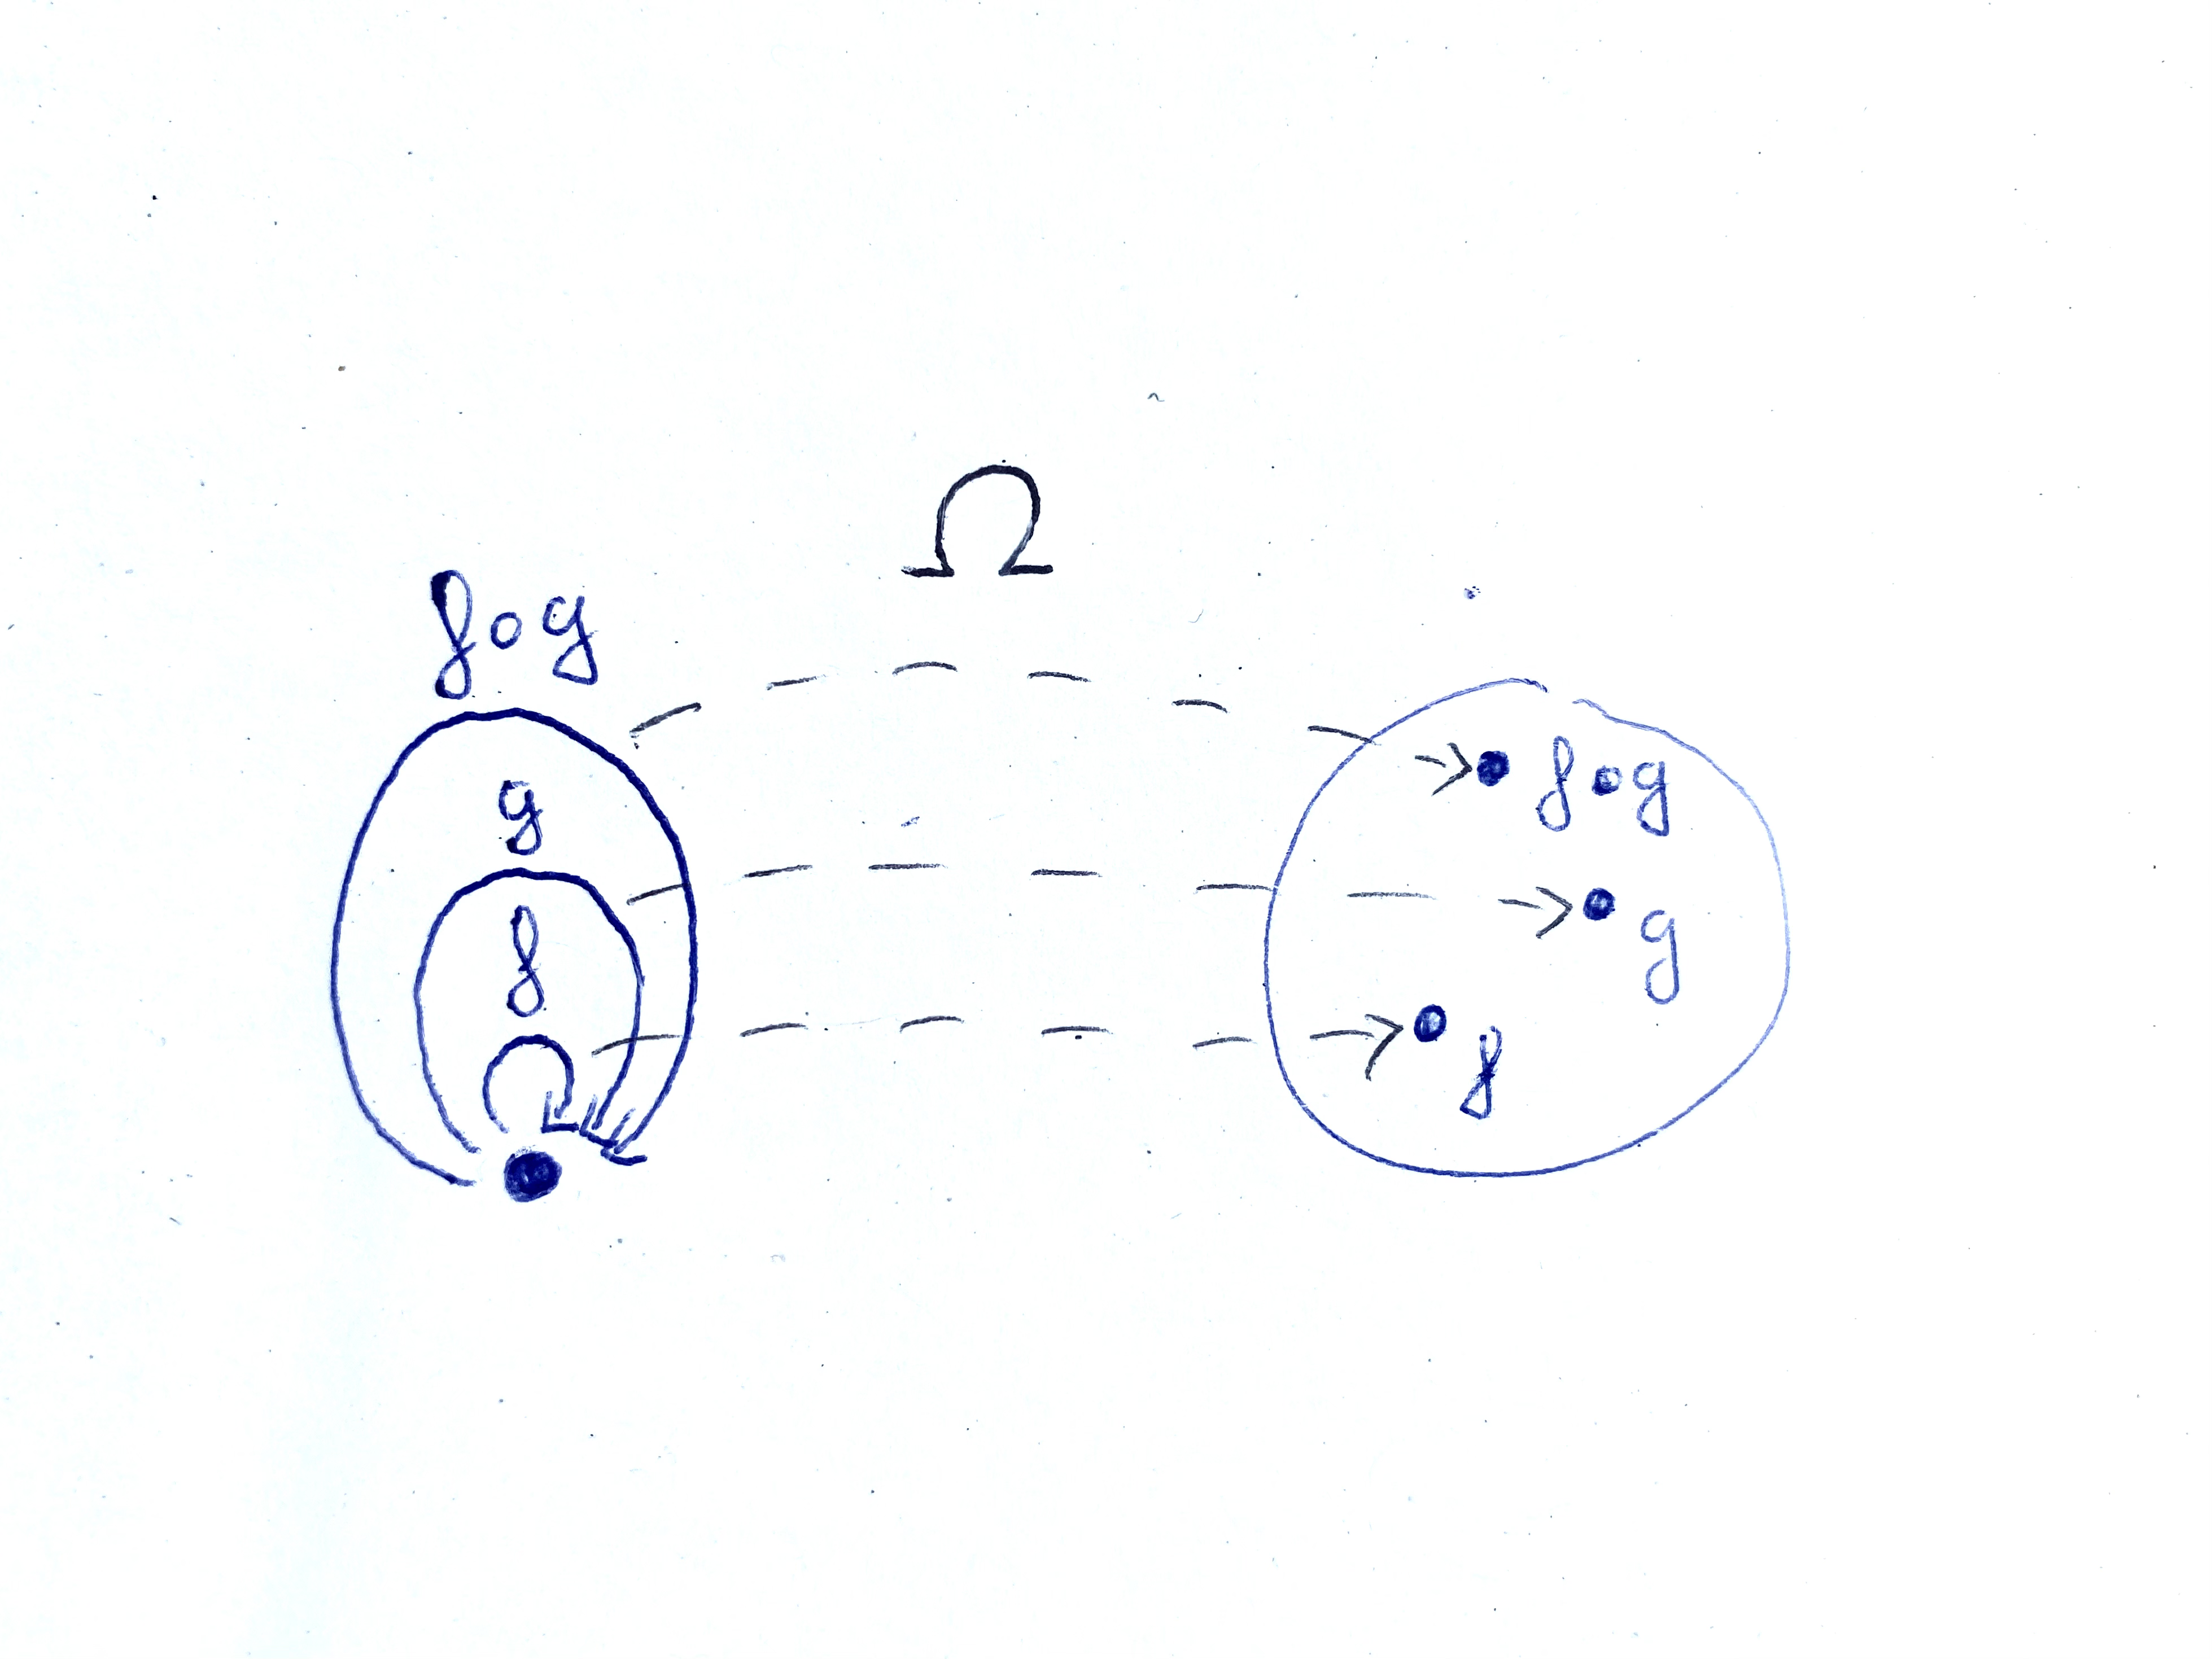
\includegraphics[scale=0.03]{omega}
% \end{figure}

Nous commencerons par quelques rappels de HoTT, afin de détailler la constructions de groupes, ainsi que les notions associées (morphismes, actions, torseurs).

\subsection{Rappels de HoTT}

\paragraph{Looping :} Un tuple $X :\equiv (A,a_0)$ est un \emph{type-pointé} si $A$ est un type et $a_0 : A$. On définit le \emph{loop-space} de ce type pointé :

\[\Omega(X) = (a_0 =_{A} a_0)\]

\paragraph{$n$-types :} On rappelle quelques notions sur la structure des égalités d'un type donné :

\begin{itemize}
  \item \emph{Proposition} : type possèdant au plus un habitant. ($\prod_{x,y : A} (x = y) $)
  \item \emph{Ensemble} : type dont les égalités sont des propositions.
  \item \emph{Groupoïde} : type dont les égalités sont des ensembles.
\end{itemize}

On note $\prop$ et $\set$ les types des propriétés et des ensembles dans un univers $\mathcal{U}$. On remarque qu'une proposition est toujours un ensemble, qu'un ensemble est un groupoïde... On parle aussi de $(-1)$-type pour les propositions, de $0$-type pour les ensembles, de $1$-types pour les groupoïdes et plus généralement de $n$-type.

\paragraph{Troncatures :} On parle de la $n$-troncature de $A$, notée $\|A\|_{n}$, pour le type satisfaisant la propriété universelle suivante :

\begin{equation*}
 INSERER \ \ DIAGRAMME
\end{equation*}

On utilisera nottement la troncature propositionnelle $\|\cdot\|_{-1}$. Intuitivement, celle-ci affirme qu'un type est non-vide sans préciser d'habitant. Cependant si ce qu'on cherche à montrer est une proposition P, on à le droit de faire comme-si on se donnait un habitant :

\[ \|A\|_{-1} \to P \simeq A \to P\]

\paragraph{Types connexes :} Dans un type connexe, tout les types égalité sont non-vides. Pour autant il ne s'agit pas toujours de propositions :

\[\prod_{x,y : X} \|x = y\|_{-1} \not\simeq \prod_{x,y : X} (x = y)\]

En particulier, une proposition (droite) a des égalités triviales, ce qui n' est pas le cas pour tout type connexe : un exemple est $\mathbb{S}_{1}$.

\subsection{Notion de Groupe en HoTT}

\begin{definition}

On appelle \emph{groupe} un tuple :

\begin{itemize}
        \item $S : Set$
        \item $e : S$
        \item $\mu : \displaystyle\sum_{\star : S \to S \to S} \displaystyle\prod_{g_1,g_2, g_3 : S} (g_1 \star e = e \star g_1 = g_1 ) \times (g_1 \star (g_2 \star g_3) = (g_1 \star g_2) \star g_3) $
        \item $\iota : \displaystyle\sum_{\inv : S \to S} \displaystyle\prod_{g : S} (f(g) \star g = g \star f(g) = e)$
\end{itemize}

\end{definition}

Un groupe est donc un ensemble muni d'une loi de composition interne associative, d'un neutre pour cette loi, et d'une fonction qui a chaque élément associe un inverse. A noter que dans la bibliographie HoTT, on appelle ce genre d'objet ``groupe abstrait'', par opposition aux groupes ``concrets'' qui sont justement les déloopings des groupes abstraits. Pour l'instant nous ne manipuleront que des groupes abstraits. On notera $\groupa$ le type des groupes abstraits.

\subsection{Morphismes et Actions de Groupes}

\begin{definition}
Si $G,H : \groupa$, une fonction $f : G \to H$ est un morphisme si elle est munie d'un témoin :

\[h : \displaystyle\prod_{x,y : G} f(x \star_{G} y) = f(x) \star_{H} f(y) \]

On note alors $(f,h) : \hom(G,H)$.
\end{definition}

\begin{definition}
Une action de (abstraite) $G \curvearrowright X$ (où $X : \set$) est une fonction :

\[\phi : G \to X \to X \]

et de témoins :

\[n : \prod_{x : X}\phi(1)(x) = x\]
\[h : \prod_{g_1, g_2 : X}\phi(g_1 \star g_2)(x) = \phi(g_1) \circ \phi(g_2) (x)\]

Et on note $\gset$ les ensembles de $\set$ munis d'une action de $G$.
\end{definition}

\begin{definition}
  On note $G$-morphisme un morphisme entre $A,B : \gset$ respectant l'action de $G$.
  On note $A \simeq_{G} B$ lorsque il existe un $G$-morphisme ayant un inverse. (un triplet avec une fonction, et les identifications des deux composées à la fonction identité). On dit que deux tels ensembles sont $G$-isomorphes.
\end{definition}

\begin{definition}
  On appelle $P_{G}$ le torseur principal de $G$, le $\gset$ de l'action (abstraite) de $G$ sur lui-même par multiplication à gauche.
\end{definition}

\section{Construction de $K(G,1)$ par torseurs}

\begin{definition}
  Si $(A,a_0)$ est un type pointé, on note $\baut(A) :\equiv \sum_{x : A}\| x = a_{0} \|_{-1}$ la composante connexe de $a_0$ dans $A$.
\end{definition}

\begin{lemme}
  Le loop-space de la composante connexe de $a_0$ est le loop-space de $a_0$ :
  \[\Omega(\baut(A)), a_0) = \Omega(A,a_0)\]
\end{lemme}

\begin{proof}
  $(\baut(A), a_0)$ est un type pointé, et soit $\code$ la fibration :
  \begin{gather*}
    \code : \baut(A)) \to \mathcal{U} \\
    (x,!) \mapsto (x =_{A} x)
  \end{gather*}
  On pose la fonction $\decode$ qui à $(x,!_{x})$ et $p : (x = a_0)$ associe un élément de :

  \[((x,!_{x}) = (a_0,!_{a_{0}})) \simeq \displaystyle\sum_{p : (x = a_0)}(p^{*}(!_{x}) = !_{a_0})\]

  Il suffit de donner un élément de ce second type. C'est un tuple, le premier élément est p, le second est une preuve de $(p^{*}(!_{x}) = !_{a_{0}})$ qu'on tire de la contractibilité de $\|a_0 = a_{0}\|_{-1}$. On vérifie les hypothèses du lemme encode-décode pour les loop-spaces :
  \begin{enumerate}
    \item $c_0 :\equiv \refl_{a_0} : \code(a_0)$
    \item $\decode : \prod_{x : \baut(A)} \code(x) \to ((a_{0},!) = x)$
    \item Si $c : \code(a_0) \equiv (a_0 = a_0)$, alors $\decode_{a_0}(c) = ((a_{0},!) = (a_{0},!))$ et :\\
          $\transport^{\code}(\decode_{a_0}(c), c_0) = c_0 \equiv \refl_{a_0}$ par construction du transport.
    \item $\decode_{a_0}(c_0) = c_{0}$
  \end{enumerate}

  Le lemme permet alors de conclure que $\Omega(BAut(A), a_0) \simeq \code(a_0) :\equiv \Omega(A,a_0)$, ce qui conclut par univalence.
\end{proof}

\begin{lemme}
  Deux ensembles $G$-isomorphes sont égaux :
    \[(A \simeq_{G} B) \simeq (A = B)\]
\end{lemme}

\begin{proof}
  On commence par montrer qu'un $G$-morphisme est un $G$-isomorphisme si et seulement si le morphisme assiocié est une équivalence (l'essentiel est de vérifier que si c'est une équivalence sa réciproque est aussi un morphisme). Nottamment ceci donne :
  \[(G \simeq_{G} H) \simeq \displaystyle\sum_{e : G \simeq H}\displaystyle\prod_{g_1,g_2 : G}e(g_1\star g_2) = e(g_1) \circ e(g_2)\]
  Par théorème, pour montrer que la famille indexée par $H : \groupa$ :
  \[ (G \simeq H) \to (G = H)\]
  Il suffit de montrer que la contractibilité de la famille :
  \[\sum_{H : \groupa} (G \simeq H) \text{  i.e.} \sum_{H : \groupa}\sum_{e : G \simeq H}\prod_{g_1,g_2 : G}e(g_1\star g_2) = e(g_1) \circ e(g_2)\]
  A FINIR
\end{proof}

\begin{lemme}
  $G \simeq (P_{G} \simeq_{G} P_{G})$
\end{lemme}

\begin{proof}
  On construit une fonction de $(P_{G} \simeq P_{G}) \to G$ et on montre que c'est une équivalence. On associe à tout $G$-morphisme $(\mu, h, e)$ l'élément $\mu(1)$. La réciproque est donc de forme $(g : G) \mapsto \cdot \star g$, qui est clairement un $G$-isomorphisme. Enfaite, tout les $G$-isomorphismes sont de cette forme car (par $h$) : $\mu(g) = g \mu(1)$.
\end{proof}

On peut à présent donner une première construction d'un délooping de $G$ :

\begin{definition}
  On pose le type des $G$-torseurs :
    \[BG :\equiv \torsor_{G} :\equiv \sum_{X : \gset}\|X = P_{G}\|\]
\end{definition}

\begin{theorem}
  L'espace des $G$-torseurs est un délooping de $G$ :
  \[\Omega(BG) \simeq G\]
\end{theorem}

\begin{proof}
  \begin{gather*}
            BG \equiv BAut((\gset, P_{G})) \\
    \Omega(BG) \simeq \Omega((\gset, P_{G})) \\
               \simeq (P_{G} = P_{G}) \\
               \simeq (P_{G} \simeq_{G} P_{G}) \\
               \simeq G
  \end{gather*}
\end{proof}

\section{Construction minimale à partir de générateurs}

Nous souhaitons à présent une construction plus simple de $BG$, on suppose qu'on dispose d'une famille génératrice $g_1, \cdots, g_{n}$ de $G$ :

\[BG =  \torsor_{g_1 \cdots g_{n}} :\equiv \sum_{X : Set} \sum_{f_1,\cdots,f_{n} : X \simeq X}\|(X,f_1,\cdots,f_{n}) = (G,\lambda x.g_1x,\cdots,\lambda x.g_{n}x)\|_{-1}\]

On va construire un inverse à la fonction :

\begin{gather*}
  eq_{1} : \torsor_{g_1 \cdots g_{n}} \to \torsor_{G}\\
        ((X,f_1, \cdots, f_{n}), e) \mapsto ([1],[2])
\end{gather*}

\paragraph{[1]} On construit un $G$-set en posant une action $\phi$ sur $X$ :

Pour tout $g = g_{i_{1}} \cdots g_{i_{r}}$ on pose $\phi(g) = f_{i_{1}} \circ \cdots \circ f_{i_{r}}$
Dont on montre rapidement qu' elle respecte la loi de groupe.

\paragraph{[2]} On veut montrer $\|X = P_{G}\|_{-1}$ qui est une propriété donc on peut utiliser :
\[p : (X,f_1,\cdots,f_{n}) = (G,\lambda x.g_1x,\cdots,\lambda x.g_{n}x)\]
C'est à dire qu'on a une équivalence $f : (X \simeq G)$ qui fait commuter pour tout $i$ :

INSERER DIAGRAMME

Et on veut une équivalence $h : (X \simeq G)$ qui fasse commuter pour tout $g$ :

INSERER DIAGRAMME

i.e.

INSERER DIAGRAMME

Ce que $f$ vérifie :

INSERER DIAGRAMME

\end{document}
